\chapter{Evaluation}
\label{cha:evaluation} Evaluation requires to define performance measures to be optimized.
The evaluation process differs from solving a classic optimization problem. Indeed,
performance of learning algorithms cannot be evaluated on entire domain. The purpose
of machine learning is to learn a model from a restricted training set and perform
generalization from this knowledge. Performance evaluation is needed for:
\begin{itemize}
	\item tuning hyperparameters of learning methods (e.g. type of kernel and kernel
		parameters, learning rate of perceptron)

	\item evaluating quality of learned predictor

	\item computing statistical significance of difference between learning algorithms
\end{itemize}

The training loss function measures the cost paid for predicting $f(x)$ for
output $y$ ($f(x)$ is the predicted value; $y$ is the ground truth). It is
designed to boost effectiveness and efficiency of learning algorithms (e.g.
\textit{hinge loss} for SVM). Typically the purpose of the training is to minimize
a training loss. As a consequence, ideal training loss functions are smooth,
differentiable. As a result, not all the performance measures can be used as
loss functions. Actually there is a difference between a loss function and the final
performance measure. For example, \textit{accuracy} (i.e. fraction of examples
correctly classified) is a performance measure which can not be used as a loss function.
More in depth, accuracy (or misclassification cost) is never used as a loss function,
since it is \textit{piecewise constant} and so not amenable to gradient descent.
A function is said to be piecewise constant if it is locally constant in
connected regions separated by a possibly infinite number of lower-dimensional
boundaries. Square wave (Figure \ref{fig:square_wave}) is an example of piecewise
constant function. This latter is not differentiable in correspondence of the
jumps and has first derivative equals to zero when it is constant. The gradient cannot
be computed or it is zero and so it does not indicate where to move in order to find
the optimum.

\begin{figure}[H]
	\centering
	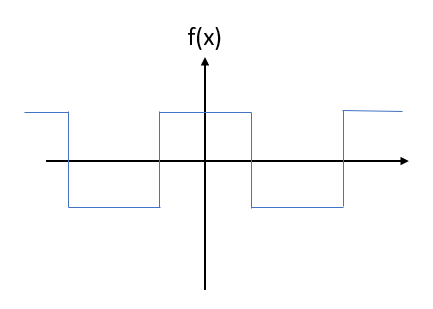
\includegraphics[width=0.5\textwidth]{
		images/06_Evaluation_squareWaveFunction.png
	}
	\caption{Square wave function is an example of piecewise constant function.}
	\label{fig:square_wave}
\end{figure}

An example of training loss function is \textit{cross entropy loss}.
\newline

Typically it is useful to consider multiple performance measures which can highlight
complementary information about the model under study.

\section{Binary classification}
\label{sec::performanceBinaryClassification} The typical way to visualize the performance
of a classification algorithm is by means of a \textit{confusion matrix}. This last
is a table which has the possible labels as rows and columns. In particular, the
rows represent the true labels for the data, while the columns report the
predicted labels. In the case of binary classification, the confusion matrix can
be exemplified as illustrated in Figure \ref{fig:binClassConfusionMatrix}.

\begin{itemize}
	\item TP $\rightarrow$ true positives: positives predicted as positives

	\item TN $\rightarrow$ true negatives: negatives predicted as negatives

	\item FP $\rightarrow$ false positives: negatives predicted as positives

	\item FN $\rightarrow$ false negatives: positives predicted as negatives
\end{itemize}

\begin{table}[ht]
	\centering
	\begin{tabular}{cc|cc|}
		\cline{3-4}                                         &   & \multicolumn{2}{c|}{prediction} \\
		\cline{3-4}                                         &   & \multicolumn{1}{c|}{P}         & N  \\
		\hline
		\multicolumn{1}{|c|}{\multirow{2}{*}{ground truth}} & P & \multicolumn{1}{c|}{TP}        & FN \\
		\cline{2-4} \multicolumn{1}{|c|}{}                  & N & \multicolumn{1}{c|}{FP}        & TN \\
		\hline
	\end{tabular}
	\caption{Confusion matrix for binary classification}
	\label{fig:binClassConfusionMatrix}
\end{table}

From the confusion matrix it is possible to compute several performance measures.

\defi{\textbf{Accuracy} \label{def:accuracy}\\ \textit{Accuracy} is the fraction of correctly labelled examples among all predictions. \begin{equation}\mathit{Acc}= \frac{\mathit{TP}+\mathit{TN}}{\mathit{TP}+\mathit{TN}+\mathit{FP}+\mathit{FN}}\end{equation}

\textbf{Remark:} accuracy is one minus the misclassification cost. }

Accuracy is not informative for strongly unbalanced datasets (typically negatives
much more than positives). For instance, if we monitor the presence of a rare
pathology in a set of people, negatives example would be much more than positives.
In this context, predictions are dominated by the larger class. As a consequence,
predicting everything as negative often maximizes the accuracy without learning nothing.
A possible solution consists of \textit{rebalancing} costs. Following this
technique, a positive example does not count as one but it counts as $\frac{N}{P}$
where $N=TN+FP$ and $P=TP+FN$. In this way, if we have 10 times more negatives,
when the model predicts a positive correctly, it does not count as one point but
it counts as 10 points.

\defi{\textbf{Precision} \label{def:precision}\\ \textit{Precision} is the fraction of positives among examples predicted as positives. \begin{equation}\mathit{Pre}= \frac{\mathit{TP}}{\mathit{TP}+\mathit{FP}}\end{equation}

It measures the precision of the learner when predicting positive. }

\textbf{Remark:} a problem of this measure is that I can improve precision by
predicting positive very rarely. For this reason a the following complementary measure
is introduced.

\defi{\textbf{Recall or Sensitivity} \label{def:recall}\\ \textit{Recall} (or \textit{sensitivity}) is the fraction of positive examples predicted as positives. \begin{equation}\mathit{Rec}= \frac{\mathit{TP}}{\mathit{TP}+\mathit{FN}}\end{equation} It measures the coverage of the learner in returning positive examples. }
Since these last two measures are complementary, i.e. when precision increases, the
recall typically decreases, it is not usually appropriate to consider them
separately. Nevertheless, in some contexts it could be reasonable to consider
recall and precision separately. Consider an in information retrieval task like:
"\textit{Give me the pages about machine learning from DISI website}". In this
case it is crucial to achieve a good precision in the first results of the
searching algorithm output. Vice versa, if we aim to develop a cancer detection
application, recall has to be prioritized.\\ For standard classification tasks,
there is a measure which combines recall and precision balancing the two aspects.

\defi{\textbf{F-measure} \label{def:fmeasure}\\ \textit{F-measure} combines precision and recall balancing the two aspects. $\beta$ is a parameter trading\-off precision and recall. \begin{equation}\mathit{F_\beta}= \frac{(1+\beta^{2})(\mathit{Pre}\cdot \mathit{Rec})}{\beta^{2}\mathit{Pre}+ \mathit{Rec}}\end{equation} }

The most common version of F-measure is the $F_{1}$-measure which sets $\beta=1$.
$F_{1}$ is the \textit{harmonic mean} of precision and recall. A good trade off between
precision and recall is needed in order to have a high value of $F_{1}$. $F_{1}$
is a good performance measure (better then accuracy) in the case of unbalanced
datasets.
\begin{equation}
	F_{1}= \frac{2(\mathit{Pre} \cdot \mathit{Rec})}{\mathit{Pre} + \mathit{Rec}}
\end{equation}
Classifiers often provide a confidence in the prediction (e.g. random forests,
margin or SVM). In these cases it is possible to improve precision and/or recall
by moving the confidence threshold for deciding if an element has to be
classified positively or negatively. With a high threshold we would maximize precision.
On the other hand, low values of threshold tend to maximize recall. By varying
threshold from min to max possible value, we obtain a curve of performance measures.
This curve can be shown plotting one measure (recall) against the complementary
one (precision) (see Figure \ref{fig:precisionRecallCurve}).

\begin{figure}[H]
	\centering
	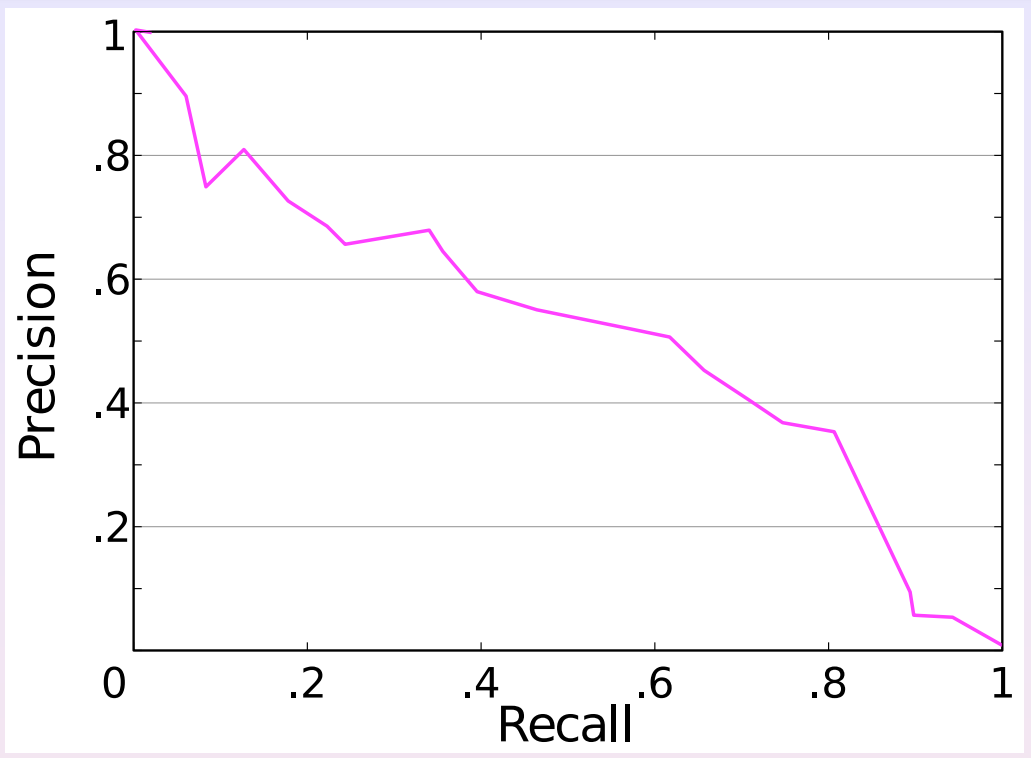
\includegraphics[width=0.5\textwidth]{
		images/06_Evaluation_precisionRecallCurve.png
	}
	\caption{Precision-recall curve. When the threshold is 0, we obtain very high
	precision, since in this case the model predicts positive only if it has very high
	confidence. On the right the graphic highlights high recall since the model
	predicts always positive with such a configuration.}
	\label{fig:precisionRecallCurve}
\end{figure}

With this tool, we can compare different algorithms by plotting them on the same
graphic. Then, we can decide the algorithm to use according to what we are
interested in.\\ A single aggregate value can be obtained taking the area under
the curve (see Figure \ref{fig:areaUnderPreRecCurve}). It combines the performance
of the algorithm for all possible thresholds (without preference for a specific
value of threshold). The area under the precision-recall curve is a good general
way to compare an algorithm with respect to another.

\begin{figure}[H]
	\centering
	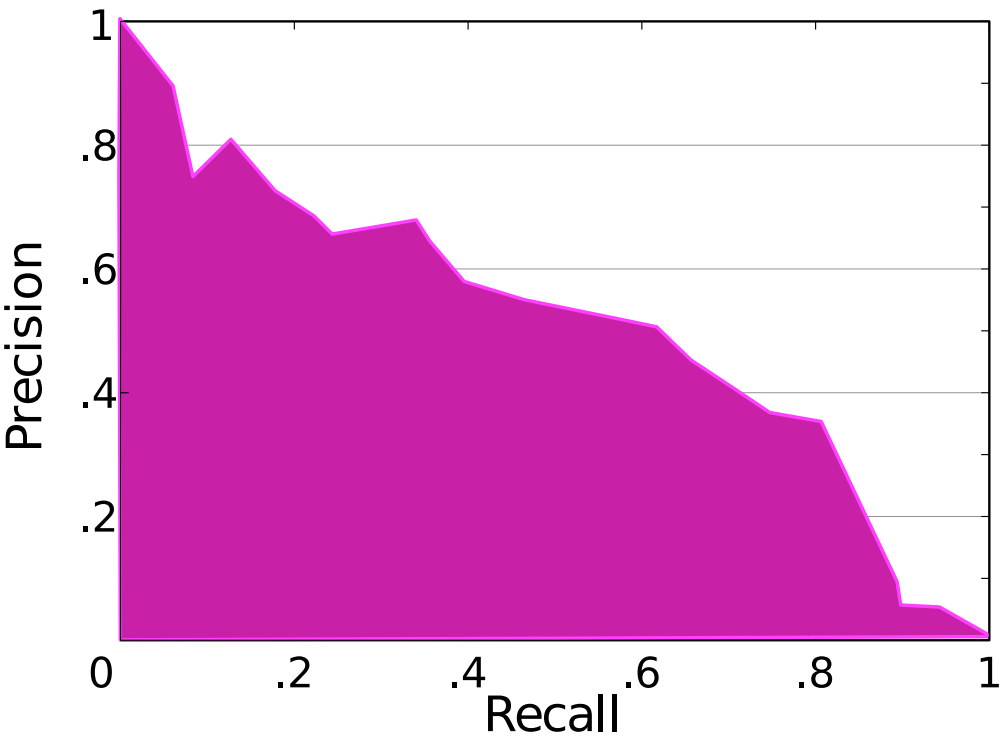
\includegraphics[width=0.5\textwidth]{
		images/06_Evaluation_areaPrecisionRecallCurve.png
	}
	\caption{Area under precision-recall curve.}
	\label{fig:areaUnderPreRecCurve}
\end{figure}

\section{Multiclass classification}
\label{sec::performanceMulticlassClassification} The notion introduced for binary
classification in Section \ref{sec::performanceBinaryClassification} can be extended
to the domain of multiclass classification.\\ The confusion matrix is a generalized
version of the binary one. The rows are the ground truth labels, while the columns
represents the predicted labels. The structure of a confusion matrix in the case
of multiclass classification is schematized in Figure
\ref{fig:confisionMatrixMulticlassClassification}.

\begin{table}[ht]
	\centering
	\begin{tabular}{cc|clc|}
		\cline{3-5}                                         &                              & \multicolumn{3}{c|}{prediction} \\
		\cline{3-5}                                         &                              & \multicolumn{1}{c|}{$y_{1}$}   & \multicolumn{1}{l|}{$y_{2}$}  & $y_{3}$                       \\
		\hline
		\multicolumn{1}{|c|}{\multirow{3}{*}{ground truth}} & $y_{1}$                      & \multicolumn{1}{c|}{$n_{11}$}  & \multicolumn{1}{l|}{$n_{12}$} & $n_{13}$                      \\
		\cline{2-5} \multicolumn{1}{|c|}{}                  & \multicolumn{1}{l|}{$y_{2}$} & \multicolumn{1}{l|}{$n_{21}$}  & \multicolumn{1}{l|}{$n_{22}$} & \multicolumn{1}{l|}{$n_{23}$} \\
		\cline{2-5} \multicolumn{1}{|c|}{}                  & $y_{3}$                      & \multicolumn{1}{c|}{$n_{31}$}  & \multicolumn{1}{l|}{$n_{32}$} & $n_{33}$                      \\
		\hline
	\end{tabular}
	\caption{Multiclass classification confusion matrix.}
	\label{fig:confisionMatrixMulticlassClassification}
\end{table}

\begin{itemize}
	\item $n_{ij}$ is the number of examples with class $y_{i}$ predicted as $y_{j}$

	\item the main diagonal contains true positives for each class

	\item the sum of off-diagonal elements along a column is the number of false positives
		for the column label:
		\[
			\mathit{FP}_{i}= \sum_{j \neq i}n_{ji}
		\]

	\item the sum of off-diagonal elements along a row is the number of false negatives
		for the row label:
		\[
			\mathit{FN}_{i}= \sum_{j \neq i}n_{ij}
		\]
\end{itemize}

At this point we can compute the performance measures discussed above in Section
\ref{sec::performanceBinaryClassification}. Accuracy, precision, recall, $F_{1}$-measure,
are defined "\textit{per-class}" (e.g. $\mathit{Pre}_{i}$ indicates the
precision of class $i$) considering as negatives examples from other classes.
\begin{itemize}
	\item Precision of class $i$
		\[
			\textit{Pre}_{i}= \frac{n_{ii}}{n_{ii}+\textit{FP}_{i}}
		\]

	\item Recall of class $i$
		\[
			\textit{Rec}_{i}= \frac{n_{ii}}{n_{ii}+\mathit{FN}_{i}}
		\]
\end{itemize}

An extension of the accuracy in a multiclass setting is the concept of \textit{multiclass
accuracy}.

\defi{\textbf{Multiclass accuracy} \label{def:multiclassAccuracy}\\ Multiclass accuracy is the overall fraction of correctly classified examples. \begin{equation}\mathit{MAcc}= \frac{\sum_{i}n_{ii}}{\sum_{i}\sum_{j}n_{ij}}\end{equation} }

In the same manner, we can compute $F_{1}$ for class $i$ and the average $F_{1}$
across classes.
\newline

From the confusion matrix we can infer the pair of classes which are often confused
by the classifier. This kind of observations could for example highlight the
need of considering additional features in order to disambiguate classes.

\section{Regression}
\textit{Root mean squared error} is the typical performance measure in the regression
domain. Intuitively, it represents the distance between the predicted value and the
real value.
\begin{equation}
	\textit{RMSE}= \sqrt{\frac{1}{n}\sum_{i=1}^{n}(f(x_{i})-y_{i})^{2}}
\end{equation}
for dataset $\mathcal{D}$ with $n=|\mathcal{D}|$.
\newline

Another useful performance parameter for regression is the \textit{Pearson
correlation coefficient}:
\begin{equation*}
	\rho = \frac{\textit{cov}(X,Y)}{\sigma_{X}\sigma_{Y}}= \frac{E[(X-\Bar{X})(Y-\Bar{Y})]}{\sqrt{E[(X-\Bar{X})^{2}E[(Y-\Bar{Y})^{2}]})]}
\end{equation*}

The random variable $X$ represents the predicted value, the random variable $Y$
represents the ground truth label. However, the expectation values can be
computed only knowing the probability distribution. This last is typically unknown
in machine learning tasks. As a consequence we approximate the expected values
considering the average value over the entire dataset.

\begin{equation}
	\rho = \frac{\sum_{i=1}^{n}(f(x_{i})-\Bar{f}(x_{i}))(y_{i}-\Bar{y_i})}{\sqrt{\sum_{i=1}^{n}(f(x_{i})-\Bar{f(x_i)})^{2}\sum_{i=1}^{n}(y_{i}-
	\Bar{y_i})^{2}}}
\end{equation}

\section{Performance estimation}
Computing performance measures on training set would be optimistically biased.
We need to rely on different approaches. A typical method to deal with these circumstances
is the \textit{Hold-out procedure}.

\subsection{Hold-out procedure}
Given a labelled training set $\mathcal{D}$, we split it in three independent sets:
\begin{itemize}
	\item \textit{Training set} (40\% $\mathcal{D}$): used to train the model

	\item \textit{Validation set} (30\% $\mathcal{D}$): used to estimate the
		performance of different algorithmic settings (i.e. hyperparameters). This
		set is used to make decisions.

	\item \textit{Test set} (30\% $\mathcal{D}$): used to estimate final
		performance of the selected model
\end{itemize}

The problematic aspect of this method is that the split of the original dataset into
the training set, validation set and test set is constant. As a consequence,
this procedure is used when a lot of data are available. On the contrary, if the
dataset is small the prediction would be inaccurate. In the case of small datasets
we need an approach whose results do not depend on the particular split.

\subsection{k-fold cross validation}
The \textit{$k$-fold cross validation} approach splits the dataset $\mathcal{D}$
in $k$ equal sized disjoint subsets $\mathcal{D}_{i}$. For each $i \in [1,k]$:
\begin{itemize}
	\item train a predictor on $\mathcal{T}_{i}= \mathcal{D}\setminus \mathcal{D}_{i}$

	\item compute score $S$ (e.g. accuracy) of predictor $L(\mathcal{T}_{i})$ on
		test set $\mathcal{D}_{i}$:
		\[
			S_{i}= S_{\mathcal{D}_i}[L(\mathcal{T}_{i})]
		\]
\end{itemize}
After this iterative procedure, return the average score across folds.
\[
	\Bar{S}= \frac{1}{k}\sum_{i=1}^{k}S_{i}
\]
In this way, the performance doesn't depend on the specific choice of the split,
because we perform multiple splits. In real application a typical value of $k$ is
$k \geq 10$.
\newline

The variance of the average score is computed assuming independent folds as follows:
\begin{equation}
	\label{variance_score}\mathit{Var}[\Bar{S}] = \mathit{Var}[\frac{S_{1}+\hdots+S_{k}}{k}
	] \approx \frac{1}{k^{2}}\sum_{j=1}^{k}\mathit{Var}[S_{j}]
\end{equation}
Notice that, the last part of the equation is not an equality. Indeed, the sets $S
_{1}, \hdots, S_{k}$ share a lot of components. At this point the variance of
the performance score on a specific fold can not be directly computed. Since we cannot
exactly compute $\mathit{Var}[S_{j}]$, we approximate it with the \textit{unbiased
variance} across folds:
\begin{equation}
	\label{variance_across_folds}\mathit{Var}[S_{j}] = \mathit{Var}[S_{h}] \approx
	\frac{1}{k-1}\sum_{i=1}^{k}(S_{i}- \Bar{S})^{2}
\end{equation}

It is not important to understand why we divide the result by $k-1$. In essence,
it is necessary because an unbiased estimate, is an estimate such that, if we consider
an infinite number of cases converges to the true prediction. If we plug
Equation \ref{variance_across_folds} into Equation \ref{variance_score}, we get:
\begin{equation}
	\mathit{Var}[\Bar{S}] \approx \frac{1}{k^{2}}\sum_{j=1}^{k}\frac{1}{k-1}\sum_{i=1}
	^{k}(S_{i}- \Bar{S})^{2}= \frac{1}{k^{2}}\frac{k}{k-1}\sum_{i=1}^{k}(S_{i}- \Bar
	{S})^{2}= \frac{1}{k}\frac{1}{k-1}\sum_{i=1}^{k}(S_{i}- \Bar{S})^{2}
\end{equation}

\section{Hypothesis testing}
We want to compare generalization performance of two learning algorithms. We
want to know whether observed difference in performance is \textit{statistically
significant} (and not due to some noisy evaluation). Hypothesis testing allows
to test the statistical significance of a hypothesis (e.g. the two predictors
have different performance).
\newline

\textbf{Null hypothesis:} $H_{0}$ default hypothesis, for rejecting which evidence
should be provided
\newline

\textbf{Test statistic:} Given a sample of $k$ realizations of random variables $X
_{1}, \hdots, X_{k}$, a \textit{test statistic} is a statistic $T=h(X_{1}, \hdots
,X_{k})$ whose value is used to decide whether to reject $H_{0}$ or not.
\newline

Example: given a set measurements $X_{1}, \hdots, X_{k}$, decide whether the actual
value to be measured is zero.
\begin{itemize}
	\item \textit{Null hypothesis:} the actual value is zero

	\item \textit{Test statistic:} sample mean:
		\[
			T = h(X_{1}, \hdots , X_{k}) = \frac{1}{k}\sum_{i=1}^{k}X_{i}= \Bar{X}
		\]
\end{itemize}

\subsection{Glossary}
\begin{itemize}
	\item \textit{Tail probability}: probability that $T$ is at least as great (right
		tail) or at least as small (left tail) as the observed value $t$.

	\item \textit{p-value}: the probability of obtaining a value $T$ at least as extreme
		as the one observed $t$, under the assumption that the null hypothesis is
		correct. A very small p-value means that such an extreme observed outcome would
		be very unlikely under the null hypothesis. (Figure \ref{fig:p_value})

	\item \textit{Type I error}: reject the null hypothesis when it's true. This
		is the most serious error. In order to minimize the type I it is common to put
		a threshold on the p-value.

	\item \textit{Type II error}: accept the null hypothesis when it's false.

	\item \textit{Critical region}: the set of random variables $X_{1}, \hdots, X_{k}$
		taken into account in the test statistic, can be visualized as a vector in a
		$n$-dimensional space. In this latter, we define a region $C$ such that if
		the vector lies in $C$ then the null hypothesis is rejected. In orther words
		the critical region represents the set of values of $T$ for which we reject the
		null hypothesis.

	\item \textit{Critical values}: values on the boundary of the critical region.
		\newline

		\textbf{Example:}\\ A common null hypothesis is the one which states that a Gaussian
		distribution $\mathcal{N}(\theta, 1)$ with variance 1 has mean value equals to
		one ($\theta = 1$). The adopted critical region to face this test statistic
		is the following one:
		\[
			C = \{(X_{1}, X_{2}, \hdots, X_{n}) : |1 - \frac{1}{n}\sum_{i=1}^{n}X_{i}|
			> \frac{1.96}{\sqrt{n}}\}
		\]
		So, the null hypothesis "$\theta = 1$" has to be rejected when the distance
		between the sample mean and 1 is larger then $\frac{1.96}{\sqrt{n}}$.

	\item \textit{Significance level}: The type 1 error and the type 2 error are not
		symmetric. Actually, the purpose of the test statistics is not to state that
		the null hypothesis is true or false, but the purpose of the test is to
		understand if the sampled data are compatible with the null hypothesis. As a
		consequence, there is high tolerance for accepting $H_{0}$, while it is rejected
		only if the sampled data are really improbable assuming $H_{0}$ is satisfied.
		This kind of balance is regulated according to a parameter $\alpha$. This latter
		is referred to as \textit{significance level}. The test must fulfil the property
		for which, the probability of rejecting the null hypothesis when it is true
		is lower then $\alpha$. In other words, the significance level $\alpha$ is
		the largest acceptable probability for committing a type 1 error. Typical values
		of $\alpha$ are $0.1, 0.05, 0.005$.
		\newline

		\textbf{Example:}\\ Suppose we want to verify the following null hypothesis:
		\[
			H_{0}: \theta \in w
		\]
		where $w$ is a set of possible values for parameter $\theta$. For this purpose,
		a point estimator $d(\pmb{X})$ is considered. The null hypothesis $H_{0}$ is
		rejected when $d(\pmb{X})$ is "far" from region $w$. In order to understand
		how much "far" $w$ and $d(\pmb{X})$ should be in order to reject $H_{0}$
		with a significance level $\alpha$, it is necessary to know the distribution
		of the estimator $d(\pmb{X})$ when $H_{0}$ is true. This notion would allow
		us to use the property such that the probability of the type 1 error is
		lower than $\alpha$, to understand when the estimator is "far" enough from $w$
		to reject the null hypothesis, and so defining the critical region of the
		test.
\end{itemize}

\begin{figure}[H]
	\centering
	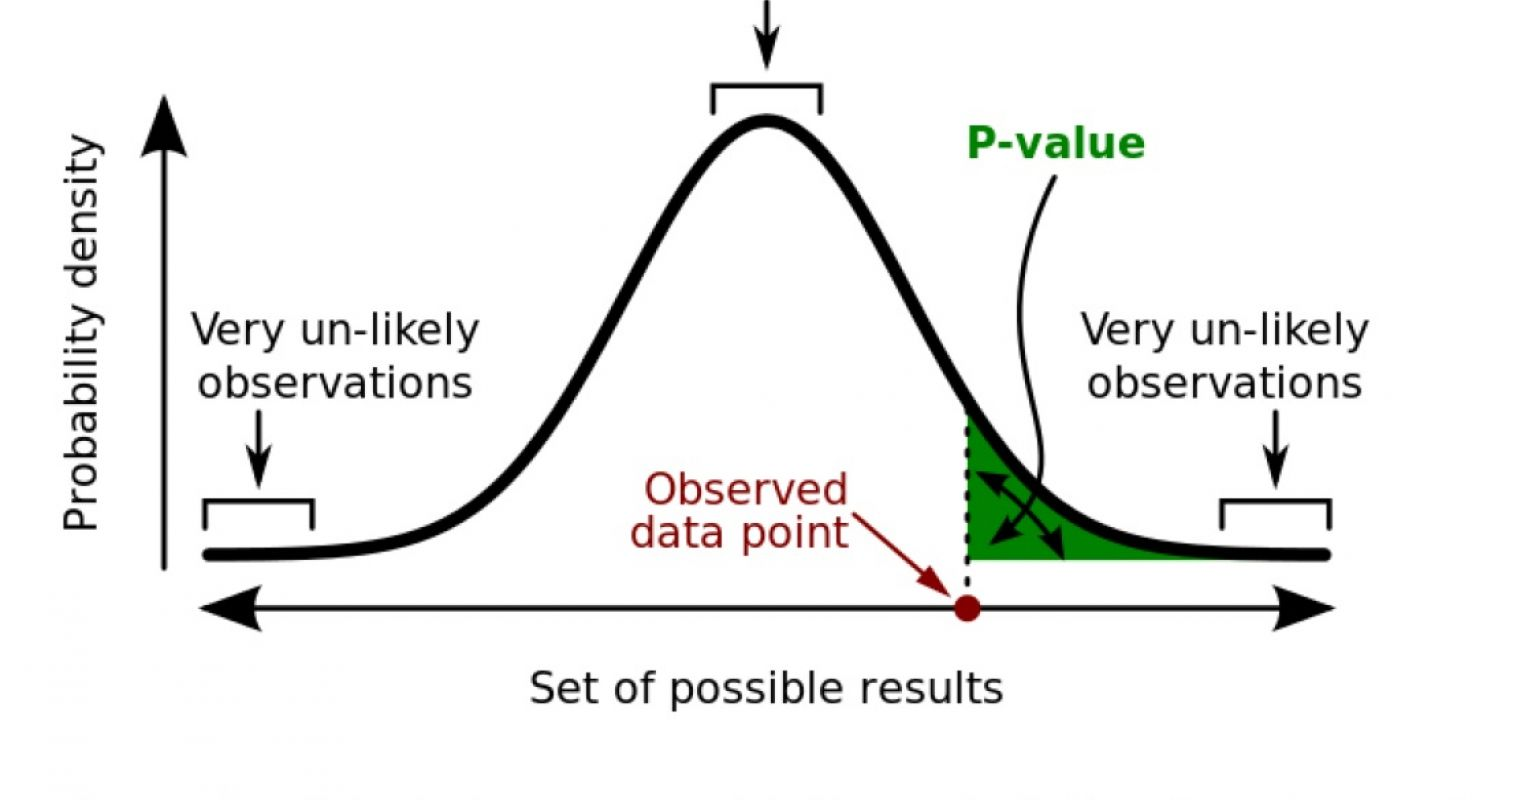
\includegraphics[width=0.8\textwidth]{
        images/06_Evaluation_pValue.jpg
    }
	\caption{p-value}
	\label{fig:p_value}
\end{figure}

\subsection{A useful digression to better understand hypothesis testing}
Suppose that $X_{1}, X_{2}, \hdots, X_{n}$ is a random sample sampled from a normal
distribution with parameters $\mu$ and $\sigma^{2}$. The variance of the normal
distribution is known, while the mean value is unknown. Given a plausible mean
value $\mu_{0}$, we want to test the null hypothesis:
\[
	H_{0}: \mu = \mu_{0}
\]

For example, if we are testing the performance differences between two machine
learning algorithms and the null hypothesis states that there is no difference
between the performance of the two algorithms, then the mean value of their difference
in performance would be 0.
\newline

In this case, $\Bar{X}:= \frac{1}{n}\sum_{i=1}^{n}X_{i}$ is the natural punctual
estimator for $\mu$. We accept $H_{0}$ when $\Bar{X}$ is not too far from
$\mu_{0}$. As a consequence, for a proper choice of the constant $c$, the critical
region is:
\begin{equation}
	\label{example_criticalRegion}C = \{(X_{1},X_{2},\hdots,X_{n}) : |\Bar{X}|-\mu_{0}
	|>c\}
\end{equation}
If our intention is to build a test with significance level $\alpha$, we need to
find the value of $c$ in Equation \ref{example_criticalRegion} such that the probability
of commit a first type error is $\alpha$. This means that $c$ has to verify the
following relation:
\begin{equation}
	\label{prob_1TypeErrorExample}\alpha = P(\mathit{I \; type \; error}) = P_{\mu_0}
	(|\Bar{X}-\mu_{0}|>c)
\end{equation}
We write $P_{\mu_0}$ to indicate the value of probability computed under the assumption
that $\mu = \mu_{0}$. Indeed, by definition, first type error occurs when the
sampled data lead us to reject $H_{0}$ (i.e. ($X_{1}, X_{2}, \hdots, X_{n}\in C$))
when indeed the null hypothesis is correct (i.e. $\mu=\mu_{0}$).\\ When
$\mu =\mu_{0}$, we know that $\Bar{X}$ is characterized by a normal distribution
with mean value $\mu_{0}$ and variance $\frac{\sigma^{2}}{n}$. Considering a
$\mathcal{N}(0,1)$ random variable $\mathcal{Z}$, we obtain:
\begin{equation}
	\frac{\Bar{X}-\mu_{0}}{\frac{\sigma}{\sqrt{n}}}\sim_{\mu_0}\mathcal{Z}
\end{equation}
Where the relation $\sim$ is conditioned to the hypothesis that: $H_{0}: \mu = \mu
_{0}$. The Equation \ref{prob_1TypeErrorExample} can now be written as:
\[
	\alpha = P_{\mu_0}(|\frac{\Bar{X}-\mu_{0}}{\frac{\sigma}{\sqrt{n}}}| > \frac{c
	\sqrt{n}}{\sigma}) = P(|Z| > \frac{c \sqrt{n}}{\sigma}) = 2P(Z > \frac{c
	\sqrt{n}}{\sigma})
\]
From this formula, we can immediately conclude that:
\[
	P(Z > \frac{c \sqrt{n}}{\sigma}) = \frac{\alpha}{2}
\]
By definition of $z_{\frac{\alpha}{2}}$ we write:
\[
	P(Z > z_{\frac{\alpha}{2}}) = \frac{\alpha}{2}
\]
From this we get:
\[
	\frac{c \sqrt{n}}{\sigma}= z_{\frac{\alpha}{2}}
\]
\[
	c = z_{\frac{\alpha}{2}}\frac{\sigma}{\sqrt{n}}
\]
We can conclude that:
\begin{itemize}
	\item if $|\frac{\Bar{X}-\mu_{0}}{\frac{\sigma}{\sqrt{n}}}|>z_{\frac{\alpha}{2}}$
		we reject $H_{0}$

	\item if $|\frac{\Bar{X}-\mu_{0}}{\frac{\sigma}{\sqrt{n}}}| \leq z_{\frac{\alpha}{2}}$
		we accept $H_{0}$
\end{itemize}
\begin{figure}[H]
	\centering
	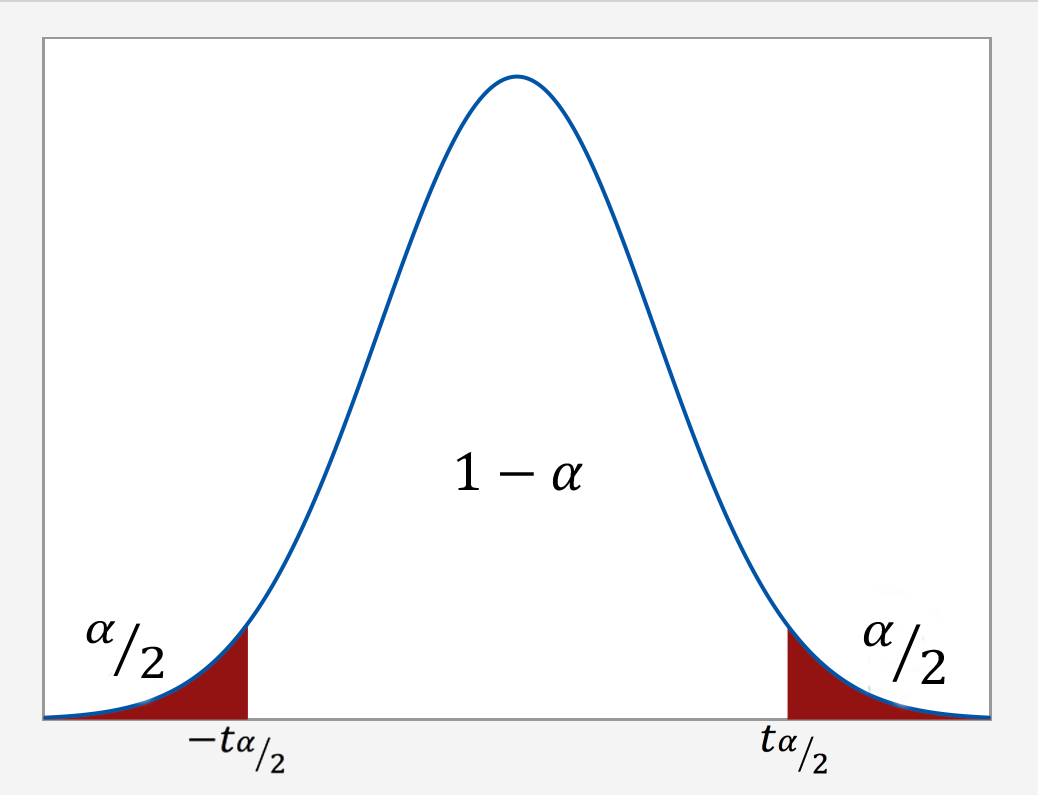
\includegraphics[width=0.5\textwidth]{
		images/06_Evaluation_normalDistributionTest.png
	}
	\caption{Confidence intervals}
	\label{fig:confidence_intervals}
\end{figure}

The acceptance region corresponds to the interval symmetric with respect to 0 labeled
with $1-\alpha$ in Figure \ref{fig:confidence_intervals}.

\subsection{Hypothesis testing when the variance is unknown}
Up to this point we have assumed that the only unknown parameter of the distribution
is the mean value. However, really often both the mean $\mu$ and the variance $\sigma
^{2}$ are unknown. Under these new assumptions, we study how to test the null hypothesis
about the mean value.
\[
	H_{0}: \mu = \mu_{0}
\]
Analogously to what we have done before, it is reasonable to reject the null hypothesis
when the sample mean $\Bar{X}$ is far from $\mu_{0}$. However, in this case the problem
is more difficult since the distance between $\Bar{X}$ and $\mu_{0}$ which determines
a rejection of the null hypothesis, depends on the standard deviation $\sigma$, which
in this new setting is unknown. In particular, in the previous case, the null
hypothesis is rejected when $|\Bar{X}-\mu_{0}|$ is larger then
$z_{\frac{\alpha}{2}}\cdot \frac{\sigma}{\sqrt{n}}$:
\[
	|\frac{\Bar{X}-\mu_{0}}{\frac{\sigma}{\sqrt{n}}}|>z_{\frac{\alpha}{2}}
\]
Since $\sigma$ is unknown, we replace it with the sample standard deviation $S$.
\begin{equation}
	S = \sqrt{\frac{1}{n-1}\sum_{i=1}^{n}(X_{i}-\Bar{X})^{2}}
\end{equation}
Given that, we reject the null hypothesis when
$|\frac{\Bar{X}-\mu_{0}}{\frac{S}{\sqrt{n}}}|$ is "too large". In order to understand
when this quantity is "too large" we need to know the distribution of the statistic
test when $H_{0}$ is verified.

\theo{\textbf{Probability distribution of a sample sampled from a Gaussian distribution with unknown variance}\label{theo:no_variance_gaussian}\\

$X_{1}, X_{2}, \hdots, X_{n}$ is a sample sampled from a Gaussian distribution with mean value $\mu$. If $\Bar{X}$ and $S^{2}$ denotes the sample average and the sample variance respectively, then: \begin{equation}\frac{\Bar{X}-\mu}{\frac{S}{\sqrt{n}}}\sim t_{n-1}\end{equation}

\begin{itemize}\item When we normalize $\Bar{X}$ by subtracting the mean value $\mu$ and dividing by the standard deviation $\frac{\sigma}{\sqrt{n}}$, we obtain a \textbf{standard normal distribution}.

\item When we normalize $\Bar{X}$ by subtracting the mean value $\mu$ and dividing by the sample standard deviation $\frac{S}{\sqrt{n}}$, we obtain a \textbf{Student's t-distribution} with $n-1$ degrees of freedom.\end{itemize} }

We denote the statistic of the test with $T$ such that:
\[
	T = \frac{\Bar{X}-\mu}{\frac{S}{\sqrt{n}}}
\]
Under the assumption that $H_{0}$ is true ($\mu = \mu_{0}$), $T$ is a $t$-distribution
with $n-1$ degrees of freedom. We impose that the probability of a type one
error is $\alpha$:
\[
	P_{\mu_0}(-c \leq \frac{\Bar{X}-\mu_{0}}{\frac{S}{\sqrt{n}}}\leq c) = 1 - \alpha
\]
\[
	\alpha = 1 - P(-c < T < c) = P(T \leq -c) + P(T \geq c) = 2P(T \geq c)
\]
\[
	P(T>c) = \frac{\alpha}{2}
\]
\[
	c = t_{\frac{\alpha}{2},n-1}
\]
In conclusion:
\begin{itemize}
	\item $H_{0}$ is rejected at a significance level $\alpha$ if:
		\[
			|\frac{\Bar{X}-\mu_{0}}{\frac{S}{\sqrt{n}}}|>t_{\frac{\alpha}{2},n-1}
		\]

	\item $H_{0}$ is accepted if:
		\[
			|\frac{\Bar{X}-\mu_{0}}{\frac{S}{\sqrt{n}}}|\leq t_{\frac{\alpha}{2},n-1}
		\]
\end{itemize}

In this case, the p-value is the probability that a Student's t-distribution
with $n-1$ degrees of freedom has a value larger then $|t|$ under the assumption
that $H_{0}$ is verified, where $t$ is the test statistic calculated from the sample
data.

\subsection{Some properties of the t distribution}
In the following we report some important properties of the $t_{k-1}$ distribution.
\begin{itemize}
	\item The Student's t-distribution is a bell-shaped distribution similar to the
		Normal one

	\item The shape is wider and shorter (fatter tails): reflects greater variance
		due to using its approximation $\tilde{Var}[\Bar{X}]$ instead of the true
		unknown variance of the distribution

	\item $k-1$ is the number of degrees of freedom of the distribution (related
		to the number of independent events observed)

	\item $t_{k-1}$ tends to the standardized normal $Z$ for $k \rightarrow \infty$
\end{itemize}

\section{Comparing learning algorithms}
The purpose of this section is to understand how to compare two learning algorithms
using hypothesis testing.\\ First of all we run k-fold cross validation procedure
for algorithms A and B. Then we compute the mean performance difference for the
two algoritms:
\begin{equation}
	\hat{\delta}= \frac{1}{k}\sum_{i=1}^{k}\delta_{i}= \frac{1}{k}\sum_{i=1}^{k}S_{\mathcal{D}_i}
	[L_{A}(\mathcal{T}_{i})] - S_{\mathcal{D}_i}[L_{B}(\mathcal{T}_{i})]
\end{equation}

Where $S_{\mathcal{D}_i}[L_{A}(\mathcal{T}_{i})]$ is the performance of
algorithm A on fold $i$. In particular the learning algorithm $L_{A}$ is executed
on a subset of the dataset ($\mathcal{T}_{i}$) while the performance ($S$) of the
algorithm is measured considering the rest of the dataset ($\mathcal{D}_{i}$).
\newline

The null hypothesis is that the mean difference is zero (i.e. there is no difference
between the two algorithms).
\[
	H_{0}: \mu = 0
\]

Clearly, the variance of the distribution is unknown. As a consequence we
implement a t-test which rejects the null hypothesis at significance level
$\alpha$ when:
\[
	\frac{\Bar{\delta}}{\sqrt{\tilde{Var}[\Bar{\delta}]}}\leq - t_{k-1, \frac{\alpha}{2}}
\]
or
\[
	\frac{\Bar{\delta}}{\sqrt{\tilde{Var}[\Bar{\delta}]}}\geq t_{k-1, \frac{\alpha}{2}}
\]
where $\Bar{\delta}$ is the sample mean of the difference and:
\[
	\sqrt{\tilde{Var}[\Bar{\delta}]}= \sqrt{\frac{1}{k(k-1)}\sum_{i=1}^{k}(\delta_{i}-
	\Bar{\delta})^{2}}
\]
Notice the the null hypothesis assumes zero means, that is why $\Bar{\delta}$ is
alone in the numerator.
\newline
We perform a two-tailed test if no prior knowledge can tell the direction of the
difference. Otherwise it is reasonable to use one-tailed test.
\subsection{t-test example: 10-fold cross validation}
In Figure \ref{fig:tTestExample} there are reported the test performances
computed on ten folds. The first column is the number of the fold ($\mathcal{D}_{1}
, \mathcal{D}_{2}, \hdots, \mathcal{D}_{10}$) of the 10-fold cross validation.
The second and the third columns reports the performances (e.g. accuracy) achieved
by algorithm A and B respectively. Finally, the fourth columns indicates the difference
between the two scores.\\ Firstly, we can easily compute the mean value of the
difference:
\[
	\Bar{\delta}= \frac{1}{10}\sum_{i=1}^{10}\delta_{i}= 0.046
\]

\begin{figure}[H]
	\centering
	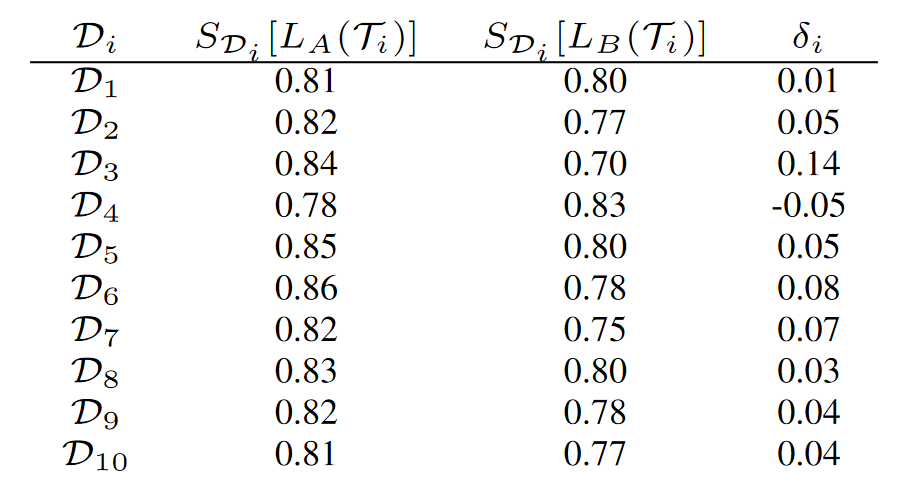
\includegraphics[width=0.8\textwidth]{
        images/06_Evaluation_tTest.png
    }
	\caption{10-fold cross validation used to implement a t-test example on the
	performance difference between two algorithms A and B.}
	\label{fig:tTestExample}
\end{figure}

At this point we compute the unbiased estimate of the standard deviation:
\[
	\sqrt{\tilde{Var}[\Bar{\delta}]}= \sqrt{\frac{1}{10 \cdot 9}\sum_{i=1}^{10}(\delta_{i}-
	\Bar{\delta})^{2}}= 0.0154344
\]
With this value we can calculate the standardized mean error difference:
\[
	\frac{\Bar{\delta}}{\sqrt{\tilde{Var}[\Bar{\delta}]}}= \frac{0.046}{0.0154344}=
	2.98
\]
We compute the $t$ distribution for $\alpha=0.05$ (i.e. we are happy to have a type
one error probability of $5\%$) (it is a two-tailed test so we consider $\frac{\alpha}{2}$
in the following formula) and $k=10$:
\[
	t_{k-1, \frac{\alpha}{2}}= t_{9,0.025}= 2.262
\]
Finally, since $2.262 < 2.98$, the null hypothesis is rejected. We can conclude
that the two classifiers are different. Indeed, my observation (i.e. my test
statistic) is further to the right with respect to $t_{k-1, \frac{\alpha}{2}}$.
In order to calculate the value of $t_{9,0.025}$ we have looked at the entry
$[d f = 9, t_{.}025]$ of the table in Figure \ref{fig:tDistributionTable}.
\newline

\begin{figure}[H]
	\centering
	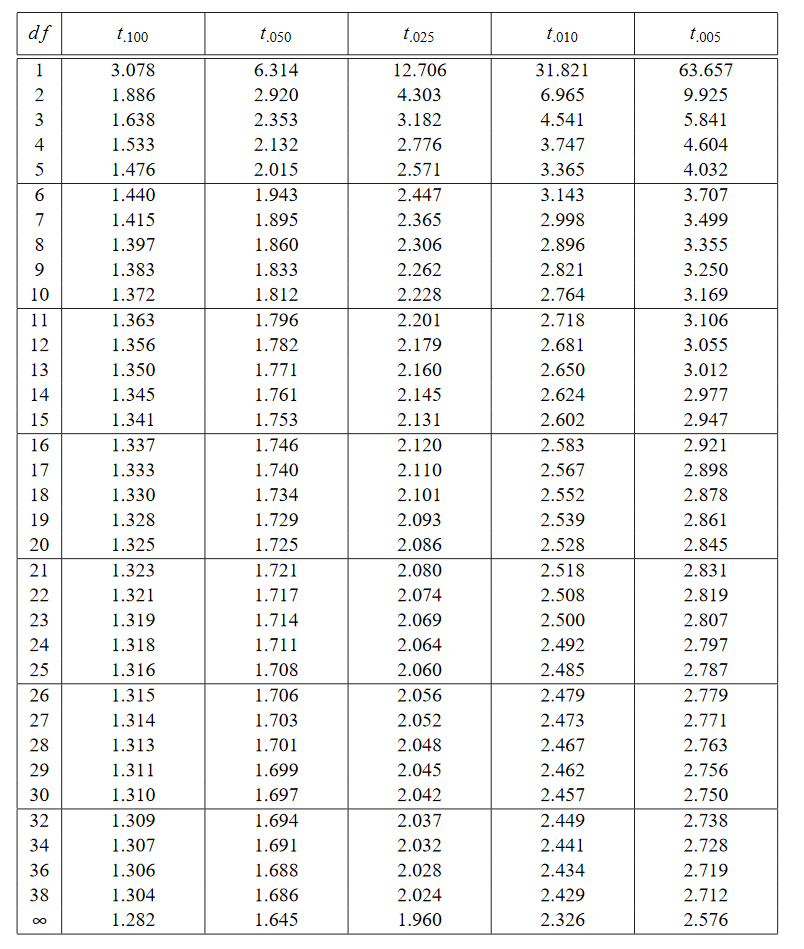
\includegraphics[width=0.6\textwidth]{
        images/06_Evaluation_tDistribution.png
    }
	\caption{Computing Student's t distribution.}
	\label{fig:tDistributionTable}
\end{figure}

\textbf{Remarks:}
\begin{itemize}
	\item The test we have described in this section is a \textit{paired test}
		since both the algorithms are evaluated over identical samples.

	\item The test we have described is a \textit{two-tailed test}. Indeed we can not
		tell a priory if algorithm A is better then B or vice versa. Otherwise, if we
		had prior knowledge about the direction of the difference, we would use a
		one-tailed test (dividing $\alpha$ by two wouldn't be required).
\end{itemize}
